\subsection{Metal-Oxide-Semiconductor Field-Effect Transistor (MOSFET)}
\markright{MOSFET}

\subsubsection*{Definition}
A MOSFET is a voltage-controlled three-terminal semiconductor device that controls
current between its \textit{drain} (D) and \textit{source} (S) terminals via the
voltage applied to its electrically insulated \textit{gate} (G) \cite{wiki:mosfet}.
The gate is separated from the semiconductor by a thin silicon dioxide ($\text{SiO}_2$)
layer, making the gate current virtually zero and giving the MOSFET an extremely high
input impedance. MOSFETs are manufactured as n-channel (NMOS) and p-channel (PMOS)
types; complementary CMOS pairs underpin all modern digital logic. The circuit symbol
and terminal labels are shown in Figure~\ref{fig:mosfet_sym}.

\theoryimage{lab-01/assets/mosfet_symbol.png}%
  {N-channel enhancement-mode MOSFET circuit symbol: the arrow on the
   body indicates n-channel type; the dashed line shows the channel forms
   only when $V_{GS} > V_{GS(\text{th})}$.}{mosfet_sym}

\begin{figure}[H]
  \centering
  \begin{subfigure}[b]{0.44\textwidth}
    \centering
    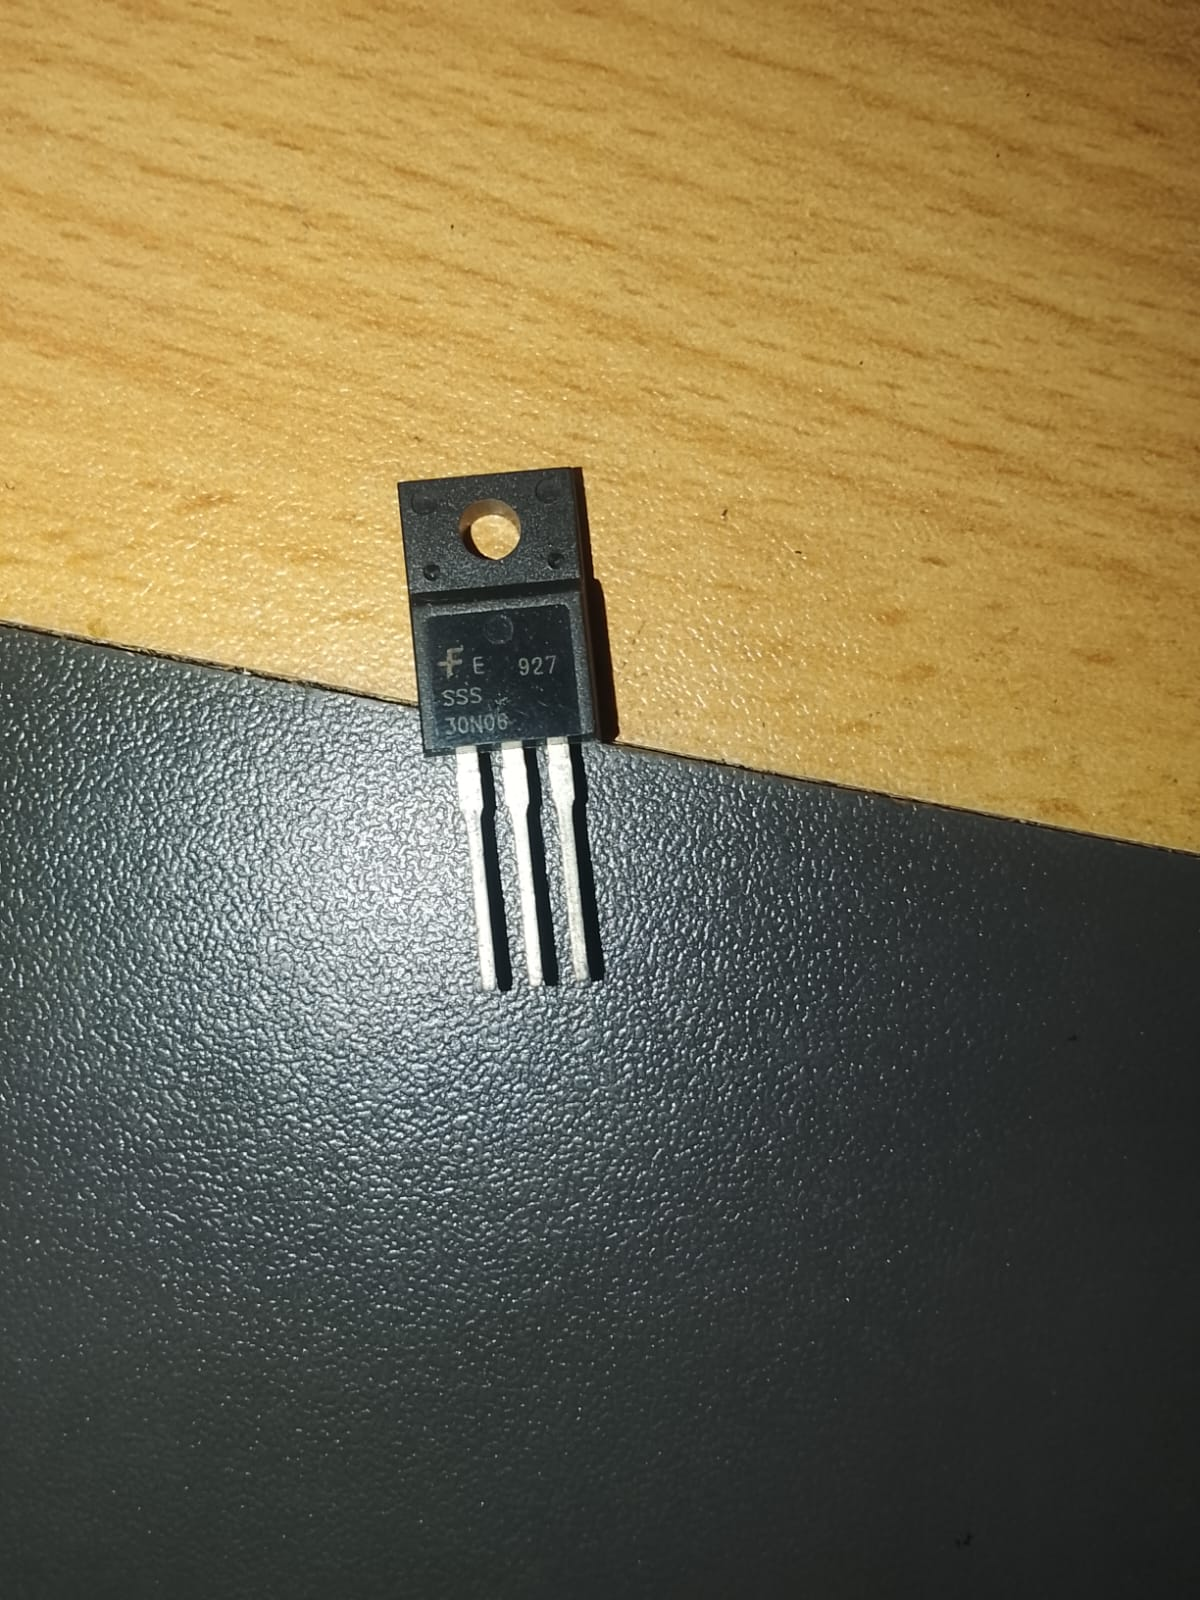
\includegraphics[width=\textwidth, height=5cm, keepaspectratio]{lab-01/assets/mosfet_to220.jpeg}
    \caption{Power MOSFET in TO-220 package}
  \end{subfigure}
  \hfill
\end{figure}

\subsubsection*{Specifications}
Key MOSFET parameters: gate threshold voltage $V_{GS(\text{th})}$ (the minimum
$V_{GS}$ to form a conducting channel), drain-to-source on-state resistance
$R_{DS(\text{on})}$ (milliohms for power devices, directly determining conduction loss),
maximum drain current $I_D$, breakdown voltage $V_{DSS}$, and transconductance $g_m$
\cite{razavi2013}. The SSS30N06 in this lab (Fairchild) is rated $I_D = 30$\,A,
$V_{DSS} = 60$\,V, $R_{DS(\text{on})} \approx 47$\,m$\Omega$.

\subsubsection*{Purpose of Use}
In the saturation region, the MOSFET is a voltage-controlled amplifier ($I_D \propto
(V_{GS}-V_{th})^2$). In the cut-off/linear (triode) region, it functions as a low-loss
electronic switch, conducting when $V_{GS} > V_{th}$ and blocking when $V_{GS} < V_{th}$.

\subsubsection*{Applications}
MOSFETs are the most produced electronic device in history. Billions of CMOS MOSFETs
constitute the logic gates in every processor, memory chip, and smartphone. Discrete
power MOSFETs switch kilowatts in motor drives, inverters, switch-mode power supplies,
and electric vehicle battery management systems \cite{wiki:mosfet}.
